\section{Thiết kế bộ nhân ma trận}

\subsection{Kiến trúc dùng 1 MAC nhân tuần tự}

Kiến trúc sử dụng một khối nhân và cộng tích lũy
(Multiply-Accumulate -- MAC) là phương án cơ bản nhất
để thực hiện phép nhân hai ma trận $8\times8$ trên FPGA.

Trong kiến trúc này, chỉ có một khối MAC được sử dụng
và được tái sử dụng nhiều lần để tính lần lượt từng phần tử
của ma trận kết quả. Ở mỗi chu kỳ tính toán, khối MAC
nhận hai toán hạng tương ứng từ ma trận $A$ và ma trận $B$,
thực hiện phép nhân, sau đó cộng kết quả vào thanh ghi tích lũy.

\begin{equation}
ACC_{k+1} = ACC_k + A_{i,k}B_{k,j},
\qquad ACC_0 = 0.
\end{equation}

Đối với ma trận $8\times8$, mỗi phần tử $C_{i,j}$ của ma trận
kết quả được tính từ tổng của 8 tích thành phần. Do đó,
sau 8 phép nhân--cộng liên tiếp, giá trị trong thanh ghi tích lũy
sẽ được ghi vào phần tử $C_{i,j}$ tương ứng. Quá trình này
được lặp lại cho đến khi tính hết 64 phần tử của ma trận kết quả.

Ưu điểm của kiến trúc này là cấu trúc đơn giản, dễ cài đặt
và thuận tiện cho việc kiểm chứng chức năng. Tuy nhiên,
do toàn bộ quá trình tính toán chỉ sử dụng một khối MAC,
các phép tính phải được thực hiện tuần tự, dẫn đến thời gian xử lý
tương đối lớn so với các kiến trúc song song.

\begin{figure}[htbp]
\centering
\resizebox{0.98\textwidth}{!}{%
\begin{tikzpicture}[
    >=Latex,
    font=\small,
    block/.style={
        draw=black!70,
        rounded corners=2pt,
        minimum width=2.3cm,
        minimum height=1.0cm,
        align=center,
        fill=white
    },
    memory/.style={
        block,
        fill=blue!8
    },
    compute/.style={
        block,
        fill=orange!12
    },
    control/.style={
        block,
        fill=green!10
    },
    line/.style={
        -{Latex[length=2.5mm]},
        thick
    },
    signal/.style={
        font=\scriptsize,
        fill=white,
        inner sep=2pt
    }
]

% Input memories
\node[memory] (brama) at (0,2)
    {BRAM A\\$A_{i,k}$};

\node[memory] (bramb) at (0,-0.2)
    {BRAM B\\$B_{k,j}$};

% Multiplier
\node[compute] (mul) at (4,0.9)
    {Multiplier\\Signed $16\times16$};

% Accumulator
\node[compute] (add) at (8,0.9)
    {Adder\\35-bit};

\node[compute] (acc) at (8,-1.5)
    {ACC Register\\35-bit};

% Output memory
\node[memory] (bramc) at (12,0.9)
    {BRAM C\\$C_{i,j}$};

% FSM
\node[control,
      minimum width=4.0cm,
      minimum height=1.1cm]
      (fsm) at (4,-4.2)
    {Controller FSM\\Counters $i,j,k$};

% Data paths
\draw[line] (brama.east) -- (2,2)
    |- (mul.west);

\draw[line] (bramb.east) -- (2,-0.2)
    |- (mul.west);

\draw[line] (mul.east) -- (add.west)
    node[midway,above,signal]{32-bit product};

\draw[line] (add.south) -- (acc.north)
    node[midway,right,signal]{Update ACC};

% Feedback from accumulator to adder
\draw[line] (acc.west) -- (6.3,-1.5)
    -- (6.3,0.3) -- (add.south west);

% Write result
\draw[line] (add.east) -- (bramc.west)
    node[midway,above,signal]{$k=7$: write result};

% FSM control paths
\draw[line,dashed] (fsm.north west)
    |- (-1.5,-2.8) -- (-1.5,2)
    -- (brama.west);

\draw[line,dashed] (fsm.west)
    -- (-1.0,-4.2)
    |- (bramb.west);

\draw[line,dashed] (fsm.east)
    -- (10.8,-4.2)
    -- (10.8,-0.5)
    |- (bramc.south);

\draw[line,dashed] (fsm.north)
    -- (4,-2.8)
    -- (8,-2.8)
    -- (acc.south);

% Controller annotation
\node[font=\scriptsize,align=center]
    at (4,-5.25)
    {$k=0\ldots7$ for each $C_{i,j}$;\\
     then advance $j$, followed by $i$};

\end{tikzpicture}%
}
\caption{Kiến trúc nhân ma trận $8\times8$
sử dụng một khối MAC tuần tự.}
\label{fig:sequential_mac}
\end{figure}

\begin{figure}[htbp]
\centering
\resizebox{0.95\textwidth}{!}{%
\begin{tikzpicture}[
    >=Latex,
    node distance=2.5cm,
    state/.style={
        draw,
        rounded corners=4pt,
        minimum width=2.0cm,
        minimum height=1.0cm,
        align=center,
        fill=blue!7,
        font=\small
    },
    arrow/.style={
        ->,
        thick,
        >=Latex
    },
    every node/.style={font=\small}
]

% States
\node[state] (idle) at (0,0) {IDLE};
\node[state] (init) at (3,0) {INIT};
\node[state] (mac) at (6,0) {MAC};
\node[state] (store) at (9,0) {STORE};
\node[state] (done) at (12,0) {DONE};

% Main transitions
\draw[arrow] (idle) -- node[above] {start} (init);
\draw[arrow] (init) -- (mac);
\draw[arrow] (mac) -- node[above] {$k=7$} (store);
\draw[arrow] (store) -- node[above] {$i=j=7$} (done);

% MAC loop
\draw[arrow]
    (mac.south) -- ++(0,-0.7)
    -- ++(1.0,0)
    -- ++(0,1.6)
    -- (mac.north east)
    node[pos=0.25,right] {$k<7$};

% Next output element
\draw[arrow]
    (store.south) -- ++(0,-1.6)
    -| node[pos=0.25,below] {Next $(i,j)$} (init.south);

% Return to idle
\draw[arrow]
    (done.north) -- ++(0,1.5)
    -| (idle.north);

\end{tikzpicture}%
}
\caption{Máy trạng thái điều khiển phép nhân ma trận
$8\times8$ sử dụng một MAC tuần tự.}
\label{fig:sequential_mac_fsm}
\end{figure}

Máy trạng thái trên gồm năm trạng thái chính:
\texttt{IDLE}, \texttt{INIT}, \texttt{MAC},
\texttt{STORE} và \texttt{DONE}.


Các trạng thái và điều kiện chuyển trạng thái
của bộ điều khiển FSM được mô tả trong
Bảng~\ref{tab:sequential_mac_fsm}.

\begin{table}[htbp]
\centering
\caption{Mô tả các trạng thái của FSM điều khiển MAC tuần tự}
\label{tab:sequential_mac_fsm}
\renewcommand{\arraystretch}{1.4}
\small
\begin{tabular}{|c|p{0.38\textwidth}|p{0.35\textwidth}|}
\hline
\textbf{Trạng thái} &
\textbf{Chức năng} &
\textbf{Điều kiện chuyển trạng thái} \\
\hline

\texttt{IDLE} &
Chờ tín hiệu bắt đầu quá trình tính toán. &
Khi \texttt{start = 1}, chuyển sang \texttt{INIT}. \\
\hline

\texttt{INIT} &
Xóa thanh ghi tích lũy $ACC$ và đặt $k=0$. &
Sau khi khởi tạo, chuyển sang \texttt{MAC}. \\
\hline

\texttt{MAC} &
Thực hiện phép nhân--cộng
$ACC \leftarrow ACC + A_{i,k}B_{k,j}$
với $k=0,\ldots,7$. &
Nếu $k<7$, tiếp tục \texttt{MAC}.
Sau khi xử lý $k=7$, chuyển sang \texttt{STORE}. \\
\hline

\texttt{STORE} &
Ghi giá trị $ACC$ vào $C_{i,j}$
và cập nhật chỉ số $i,j$. &
Nếu còn phần tử chưa tính, chuyển sang \texttt{INIT}.
Ngược lại, chuyển sang \texttt{DONE}. \\
\hline

\texttt{DONE} &
Phát tín hiệu hoàn thành phép nhân ma trận. &
Chuyển về \texttt{IDLE} để chờ lần tính toán tiếp theo. \\
\hline

\end{tabular}
\end{table}
Trong sơ đồ trên, quá trình tính toán chỉ bắt đầu
sau khi toàn bộ dữ liệu của hai ma trận đầu vào
đã được nạp và lưu trữ vào BRAM. Bộ điều khiển trung tâm có nhiệm vụ điều phối
thứ tự thực thi, phát tín hiệu điều khiển đọc/ghi bộ nhớ
và cập nhật các chỉ số $i$, $j$, $k$ tương ứng với
hàng, cột và chỉ số tích lũy.

\subsubsection{Thiết kế đường dữ liệu}
\begin{figure}[htbp]
\centering
\resizebox{0.98\linewidth}{!}{%
\begin{tikzpicture}[
    x=1mm, y=1mm, >=stealth,
    font=\normalfont\small,
    mem/.style={draw, thick, rounded corners=1pt, fill=blue!6},
    reg/.style={draw, thick, fill=green!7},
    logic/.style={draw, thick, fill=orange!9},
    bus/.style={->, thick},
    ctrl/.style={->, dashed, thin},
    pin/.style={font=\scriptsize},
    name/.style={font=\small\bfseries}
]

% ==========================================================
% Tầng trên: đọc hai toán hạng và tạo tích có dấu
% ==========================================================

% RAM A và RAM B
\path[mem] (0,44) rectangle (25,58);
\node[name] at (12.5,53.5) {RAM A};
\node at (12.5,48) {$64\times16$ bit};

\path[mem] (0,22) rectangle (25,36);
\node[name] at (12.5,31.5) {RAM B};
\node at (12.5,26) {$64\times16$ bit};

\node[pin,above] at (12.5,58) {Địa chỉ $\{i,k\}$};
\node[pin,below] at (12.5,22) {Địa chỉ $\{k,j\}$};

% Thanh ghi toán hạng
\path[reg] (39,44) rectangle (65,58);
\node at (52,53.5) {\texttt{a\_data}};
\node[pin] at (52,48) {16 bit có dấu};

\path[reg] (39,22) rectangle (65,36);
\node at (52,31.5) {\texttt{b\_data}};
\node[pin] at (52,26) {16 bit có dấu};

\draw[bus] (25,51) -- (39,51);
\draw[bus] (25,29) -- (39,29);

% Một tín hiệu READ điều khiển cả hai thanh ghi
\node[pin,anchor=east] at (49,40) {\texttt{READ}};
\draw[thin,dashed] (50,40) -- (55,40);
\fill (55,40) circle (0.55mm);
\draw[ctrl] (55,40) -- (55,44);
\draw[ctrl] (55,40) -- (55,36);

% Bộ nhân với hai ngõ vào riêng
\path[logic] (82,32) rectangle (104,48);
\node at (93,42.5) {\Large $\times$};
\node[pin] at (93,36) {signed $16\times16$};

\draw[bus] (65,51) -- (74,51) |- (82,45);
\draw[bus] (65,29) -- (74,29) |- (82,35);

% Mở rộng dấu bằng dây nối
\path[logic] (119,32) rectangle (146,48);
\node at (132.5,42.5) {Mở rộng dấu};
\node[pin] at (132.5,36) {$32\rightarrow35$ bit};

\draw[bus] (104,40) -- node[pin,above] {32 bit} (119,40);

% ==========================================================
% Tầng dưới: cộng, chọn dữ liệu, chốt ACC và ghi RAM C
% Đọc tầng này từ phải sang trái theo chiều mũi tên.
% ==========================================================

% Bộ cộng: tích mới vào từ trên, tổng cũ vào từ dưới
\node[circle,draw,thick,fill=orange!9,minimum size=9mm,
      inner sep=0pt] (adder) at (132.5,0) {\Large $+$};

\draw[bus] (132.5,32) --
    node[pin,right] {\texttt{extended\_product}[34:0]}
    (adder.north);

% MUX trước ngõ D của ACC
\path[logic] (85,-4) -- (101,-8) -- (101,8) -- (85,4) -- cycle;
\node[pin] at (93,0) {MUX};

\draw[bus] (adder.west) -- (110,0) |- (101,4);
\node[pin,above] at (116,0) {Tổng mới};

\node[pin,anchor=west] at (104,-7) {$35'd0$};
\draw[bus] (108,-4) -- (101,-4);

% Thanh ghi tích lũy
\path[reg] (48,-8) rectangle (72,8);
\node[name] at (60,2) {ACC};
\node[pin] at (60,-3.5) {35 bit};
\node[pin,anchor=east] at (71,0) {D};
\node[pin,anchor=west] at (49,0) {Q};

\draw[bus] (85,0) -- (72,0);

% RAM kết quả
\path[mem] (0,-8) rectangle (26,8);
\node[name] at (13,2.5) {RAM C};
\node[pin] at (13,-3.5) {$64\times35$ bit};

% Q của ACC vừa cấp RAM C vừa hồi tiếp về bộ cộng
\draw[bus] (48,0) -- (26,0);
\fill (37,0) circle (0.65mm);
\draw[bus] (37,0) -- (37,-20)
    -- node[pin,below] {Hồi tiếp từ Q của ACC, 35 bit}
       (132.5,-20) -- (adder.south);

% Tín hiệu ghi RAM C
\draw[ctrl] (13,-17) -- (13,-8);
\node[pin,below] at (13,-17) {\texttt{WE = STORE}};
\node[pin,above] at (13,8) {Địa chỉ $\{i,j\}$};

\end{tikzpicture}%
}
\caption{Đường dữ liệu mức RTL của bộ nhân ma trận dùng một MAC.
Nét liền biểu diễn đường dữ liệu, nét đứt biểu diễn tín hiệu điều khiển.}
\label{fig:baseline_datapath}
\end{figure}

Để giải thích độ trễ của kiến trúc cơ sở, cần xác định đường đi của
toán hạng và thời điểm kết quả được lưu tại mỗi cạnh clock.
Sơ đồ datapath là sơ đồ cần thiết để cho thấy hai toán hạng được đọc đồng thời từ RAM, 
Từ đó, có thể xác định chu kỳ, các tín hiệu waveform, signal, để thuận tiện cho việc viết testbench

Hình~\ref{fig:baseline_datapath} thể hiện datapath trong kiến trúc nhân cơ sở. Ở đây, toán hạng từ 
từ RAM A và RAM B đến bộ nhân. Tại đầu ra của ACC, dữ liệu tách thành hai nhánh: một nhánh hồi tiếp về bộ cộng để tích lũy tích tiếp theo, như đã giải thích ở kiến trúc phía trên, một nhánh cấp giá trị cho RAM C. Các phần tử toán hạng sử dụng ba chỉ số $i$, $j$, $k$ để chọn địa chỉ và điều phối ba thao tác chính trong việc đọc để xác định vị trí toán hạng

\begin{itemize}
    \item \textbf{Đọc toán hạng (\texttt{READ}).}
    Giữ cố định hàng $i$ và cột $j$. Tại cạnh lên của clock,
    hai thanh ghi \texttt{a\_data} và \texttt{b\_data} đồng thời
    nhận $A_{i,k}$ và $B_{k,j}$ từ các địa chỉ $8i+k$ và $8k+j$.

    \item \textbf{Nhân và tích lũy (\texttt{MAC}).}
    Bộ nhân tạo tích có dấu 32 bit. Tích được mở rộng dấu lên 35 bit
    rồi cộng với giá trị hồi tiếp từ ACC. Bộ nhân và bộ cộng nằm trên
    cùng một đường tổ hợp. Tại cạnh lên kế tiếp, ACC chốt tổng mới.
    Nếu $k<7$, bộ điều khiển tăng $k$ rồi quay về \texttt{READ};
    nếu $k=7$, bộ điều khiển chuyển sang \texttt{STORE}.

    \item \textbf{Ghi kết quả (\texttt{STORE}).}
    Lúc này ACC chứa tổng của cả tám tích. Tại cùng một cạnh lên,
    RAM C ghi giá trị đang có ở đầu ra ACC vào địa chỉ $8i+j$,
    còn thanh ghi ACC nhận giá trị 0 để chuẩn bị cho phần tử tiếp theo.
\end{itemize}

Mỗi phần tử $C_{i,j}$ cần $8\times2+1=17$ chu kỳ. Cụ thể, chu kỳ
thứ 16 chốt tổng cuối vào ACC và chu kỳ thứ 17 ghi tổng đó vào RAM C.
Vì bộ MAC xử lý tuần tự 64 phần tử, khoảng thời gian từ khi nhận
lệnh bắt đầu đến khi ghi $C_{7,7}$ là $64\times17=1\,088$ chu kỳ,
tương ứng $21{,}76\,\mu\mathrm{s}$ ở tần số 50~MHz.

\subsection{Cơ sở của việc tính toán song song và tái sử dụng dữ liệu}

\begin{itemize}
    \item \textbf{Tăng tốc độ tính toán}. Mỗi phần tử của ma trận kết quả \textit{C} được tính từ một hàng của \textit{A} và một cột của \textit{B}. Do các phần tử kết quả có thể được tính độc lập, việc thiết kế để các phần tử có thể tính toán song song sẽ giúp giảm thời gian tính toán ma trận đích.
    \item \textbf{Giảm lượt truy cập bộ nhớ}. Một phần tử của \textit{A} được dùng để tính nhiều phần tử trên cùng một hàng của \textit{C}, nên nhiều PE có thể cần cùng một toán hạng. Nếu mỗi PE gửi yêu cầu đọc riêng tới cùng một bank RAM, các yêu cầu có thể phải chờ do số cổng đọc của bank có hạn. Thiết kế đọc toán hạng một lần, lưu tạm rồi cấp cho các PE cần dùng.
\end{itemize}

Việc thiết kế kiến trúc tối sẽ tập trung vào hai phần: tối ưu việc \textbf{tính toán song song} và tăng mức \textbf{tái sử dụng lại dữ liệu} để tránh việc phải truy cập dữ liệu nhiều lần trên BRAM.

\subsection{Kiến trúc tối ưu}

\subsubsection{Thiết kế PE Array}

\begin{enumerate}[label=\alph*.]
    \item \textbf{Lý do chọn tile $2\times2$}

    Ma trận kết quả \textit{C} có 64 phần tử có thể tính độc lập. Nếu bố trị 1 bộ nhân riêng (DSP) cho từng phần tử thì cần 64 bộ nhân, trong khi FPGA \textbf{EP4CE6E22C8} có \textbf{15 bộ nhân chuyên dụng} phù hợp với toán hạng 16-bit. Đề tài chọn chia \textit{C} thành 16 tile $2\times2$ và bố trí mỗi tile 1 đơn vị xử lý PE. Các PE có thể tính các tile đồng thời, còn bên trong mỗi PE một bộ nhân được dùng lần lượt cho bốn phần tử của tile. Cách tổ chức này tạo được mức song song giữa các tile với tổng cộng 16 bộ nhân (15 DSP và 1 logic).

    Việc chia tile cũng tạo điều kiện cho việc tái sử dụng toán hạng. Giữa các PE, những khối cùng hàng có thể dùng chung tile của \textit{A}, những khối cùng cột có thể dùng chung tile của \textit{B}.
    
    \item \textbf{Tổ chức và phân công mảng PE}

    Mảng gồm ($4\times4$) PE. Với ($r,c \in {0,1,2,3}$), $PE_{r,c}$ phụ trách tile $C_{r,c}$, gồm các hàng (2r,2r+1) và các cột (2c,2c+1) của ma trận \textit{C}. Chẳng hạn, $PE_{2,1}$ tính bốn phần tử $C_{4,2}$, $C_{4,3}$, $C_{5,2}$ và $C_{5,3}$, như minh họa dưới đây.
    
\begin{figure}[H]
        \centering
        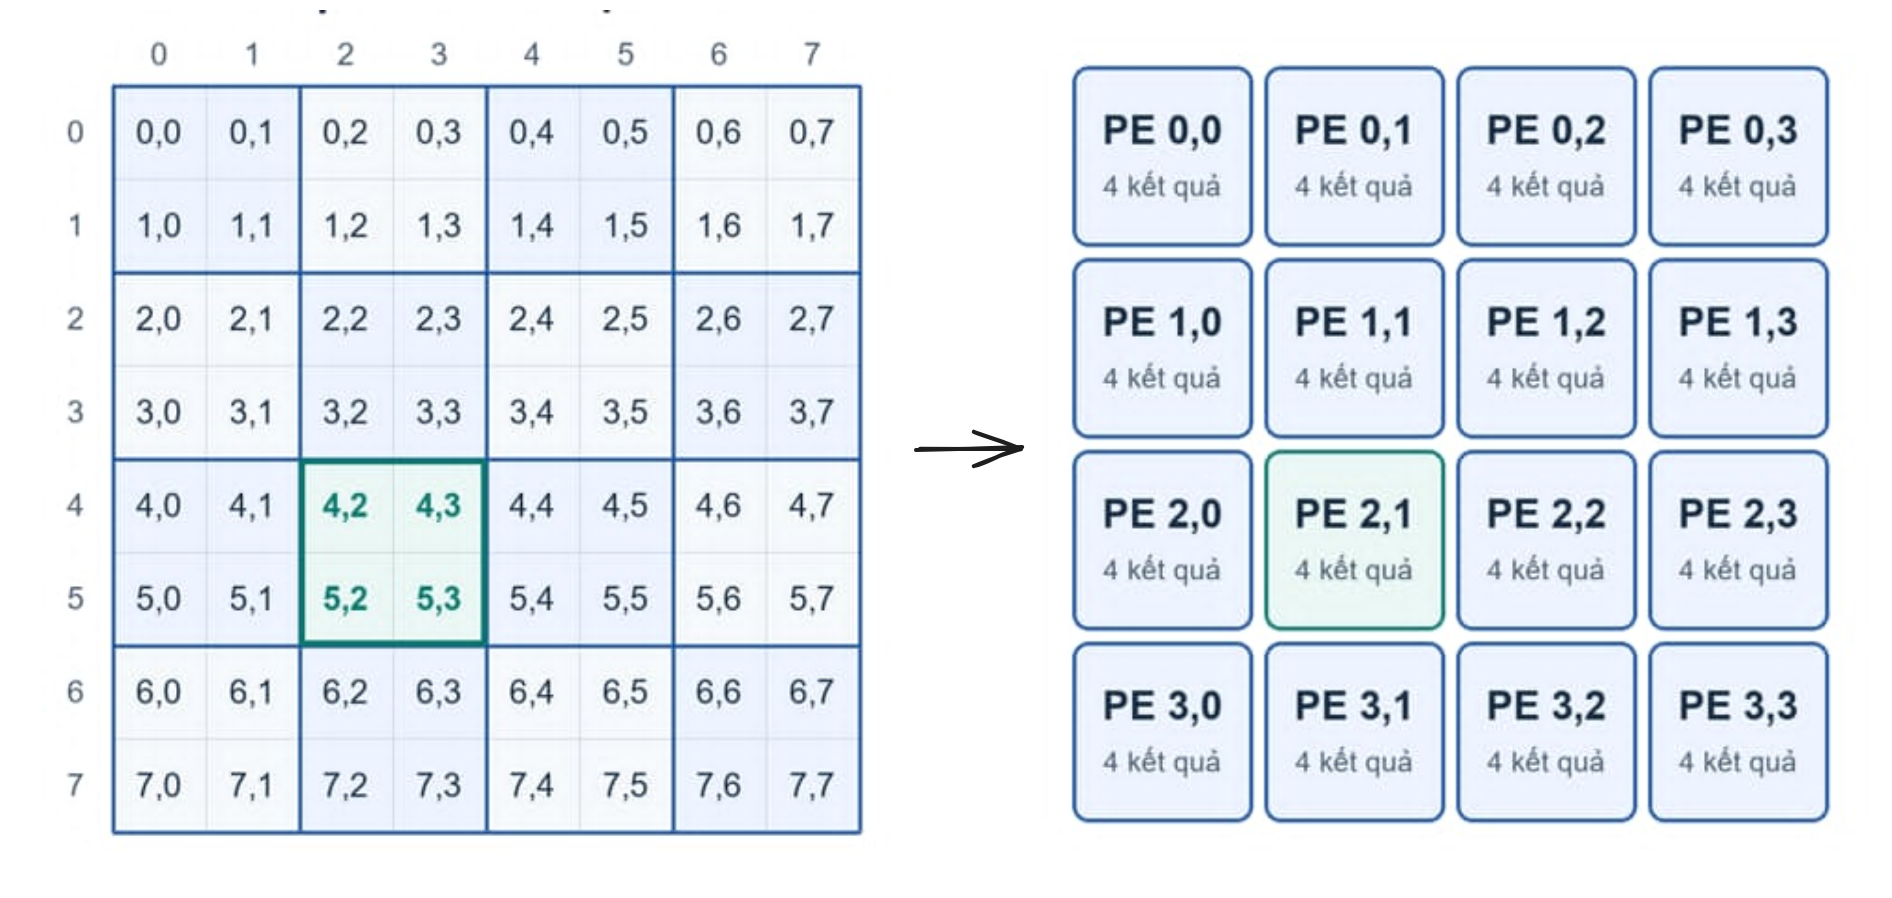
\includegraphics[width=1.0\linewidth]{figures/PE_4x4.png}
        \caption{Mảng PE 4x4}
        \label{fig:placeholder}
    \end{figure}
        
\end{enumerate}

\subsubsection{Phiên bản 1 - Systolic}

Phiên bản Systolic có 16 PE chia thành mảng ($4\times4$). Mỗi PE phụ trách 1 tile kết quả ($2\times2$). Để tái sử dụng các toán hạng, các tile của \textit{A} được truyền giữa các PE trên cùng hàng, còn các tile của \textit{B} được truyền giữa các PE trên cùng cột. Bộ điều khiển phát tile theo lịch lệch nhịp để hai toán hạng tương ứng đến đúng PE trong cùng 1 chu kỳ.

\begin{enumerate}[label=\alph*.]
    \item \textbf{Sơ đồ khối tổng thể}

    Hai ma trận đầu vào được lưu trong 2 bank BRAM đọc đồng bộ. Mỗi bank gồm 16 phần tử, mỗi phần tử chứa 1 tile ($2\times2$) độ rộng 64 bit. Cổng nạp chọn BRAM đích và địa chỉ tile. Khi cả 2 ma trận được nạp đủ, hệ thống có thể nhận lệnh \textit{start}.

    Trong mỗi lượt \textit{K}, bộ điều khiển đọc bốn tile \textit{A} và bốn tile \textit{B} vào các bộ đệm ở biên mảng. Mảng PE nhận các tile từ bộ đệm, thực hiện phép nhân tích lũy và giữ tổng riêng trong RAM cục bộ, Sau lượt cuối, bộ điều khiển chọn PE và vị trí tương ứng để lưu từng phần tử \textit{C}.
    
\begin{figure}[H]
    \centering
    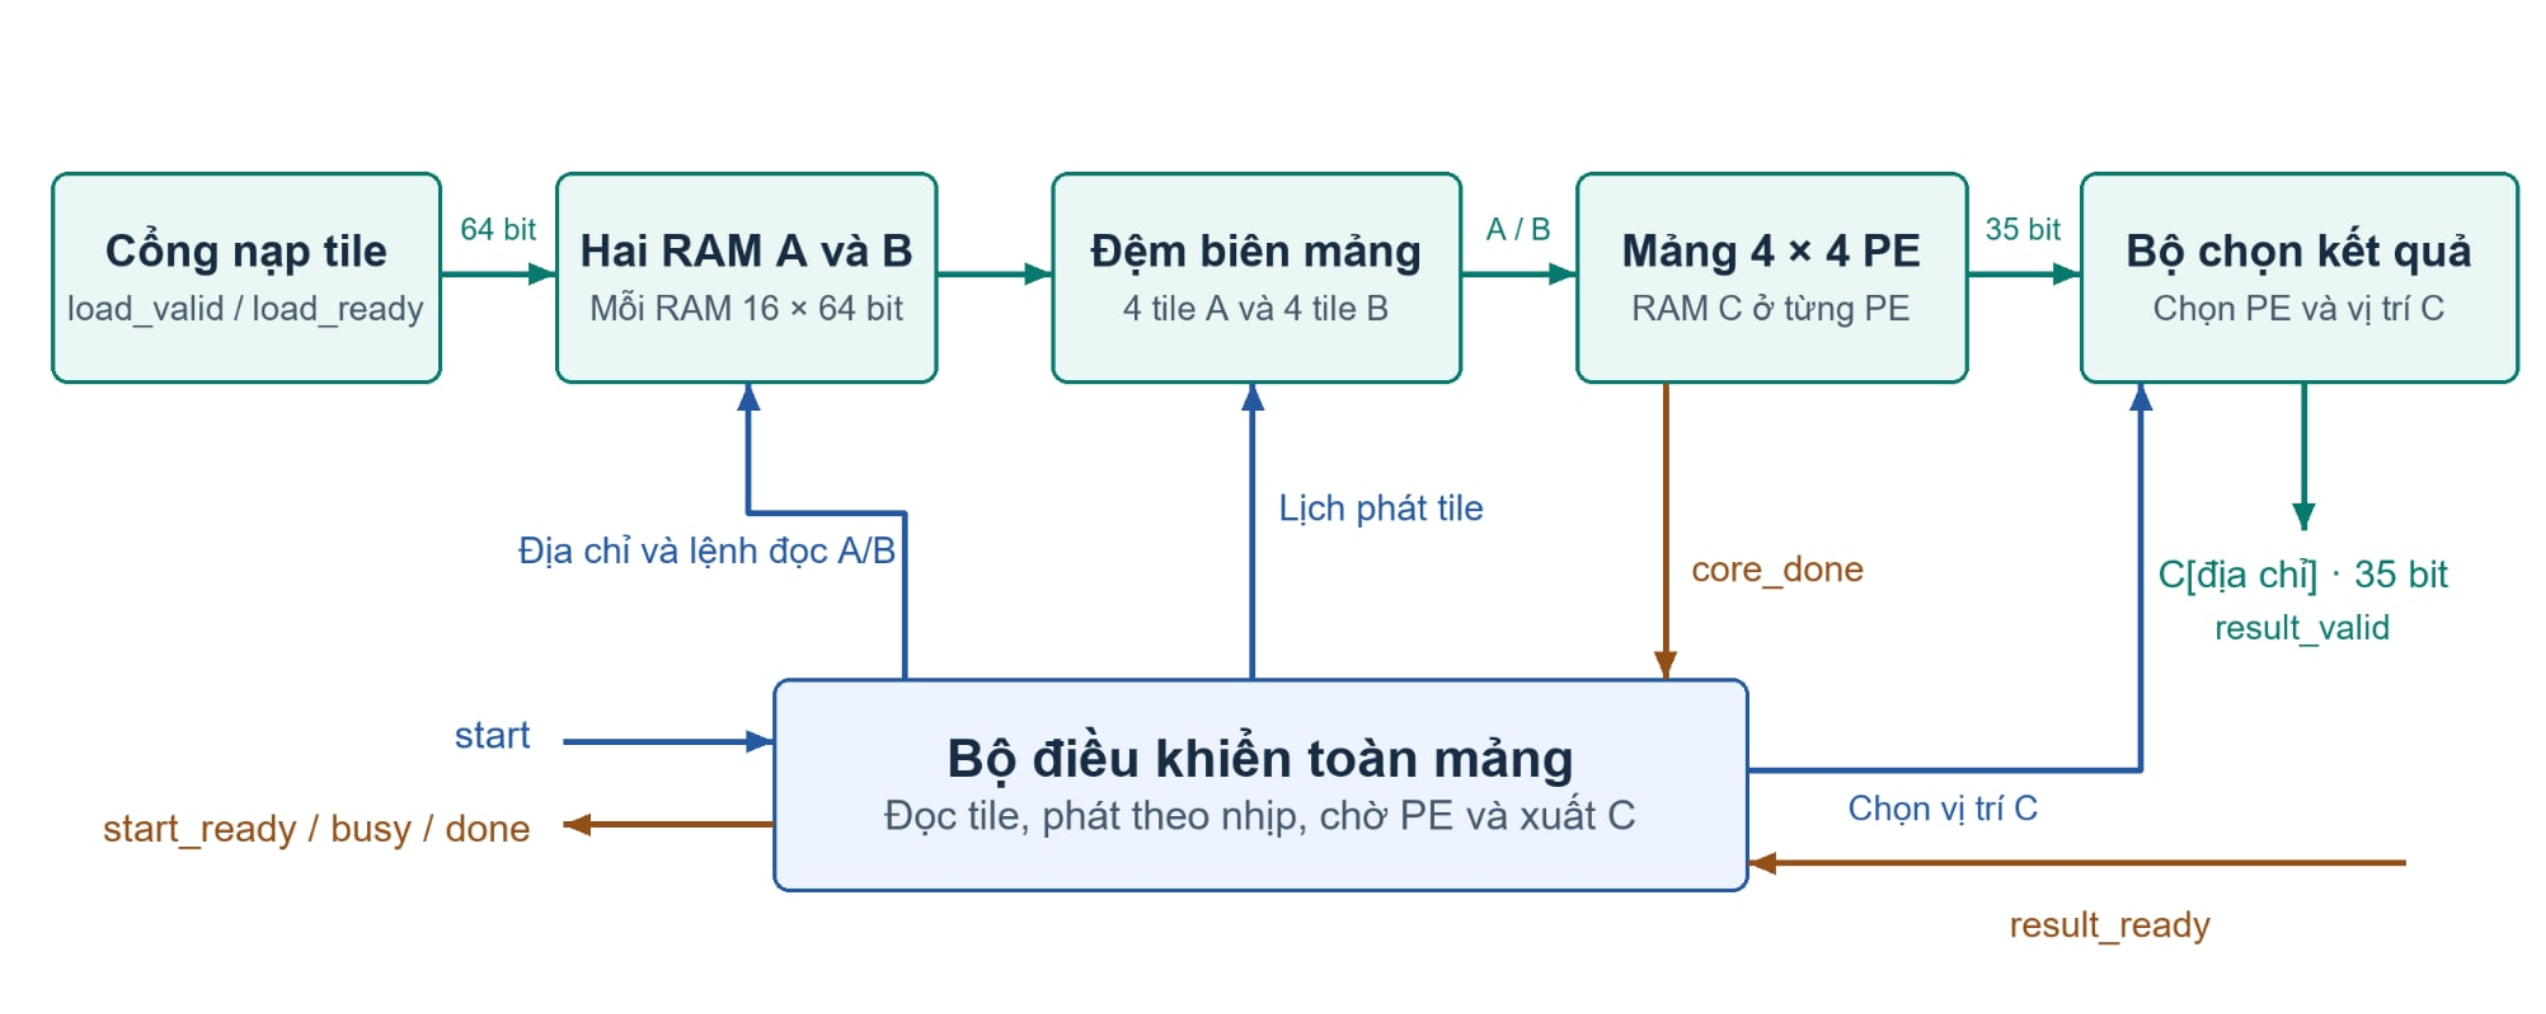
\includegraphics[width=1.0\linewidth]{figures/Systolic_block_diagram.png}
    \caption{Sơ đồ khối bộ nhân ma trận Systolic}
    \label{fig:placeholder}
\end{figure}

    \item \textbf{Kiến trúc phần cứng}

    Với cách đánh số tile theo hàng, tile tại vị trí (r,c) có địa chỉ (4r+c). Ở lượt \textit{K}, bộ điều khiển lần lượt đọc các cặp $A_{s,K}$, $B_{K,s}$. với ($s=0,1,2,3$). Hai bank BRAM được đọc đồng thời cho từng cặp. Địa chỉ đọc RAM \textit{A} là ($4s+K$), còn địa chỉ đọc RAM \textit{B} là ($4K+s$).

    Các tile \textit{A} đi vào từ mép trái và được chuyển sang PE bên phải. Các tile \textit{B} đi vào từ mép trên và được chuyển xuống PE bên dưới. Khi nhận đủ hai tile, mỗi PE chốt dữ liệu để tính toán và chuyển tiếp tile cho PE lân cận ở chu kỳ sau. Quá trình chuyển tiếp diễn ra trong khi PE đang tính. Tổng riêng của tile \textit{C} được giữ tại PE phụ trách qua bốn lượt \textit{K}.
    
\begin{figure}[H]
    \centering
    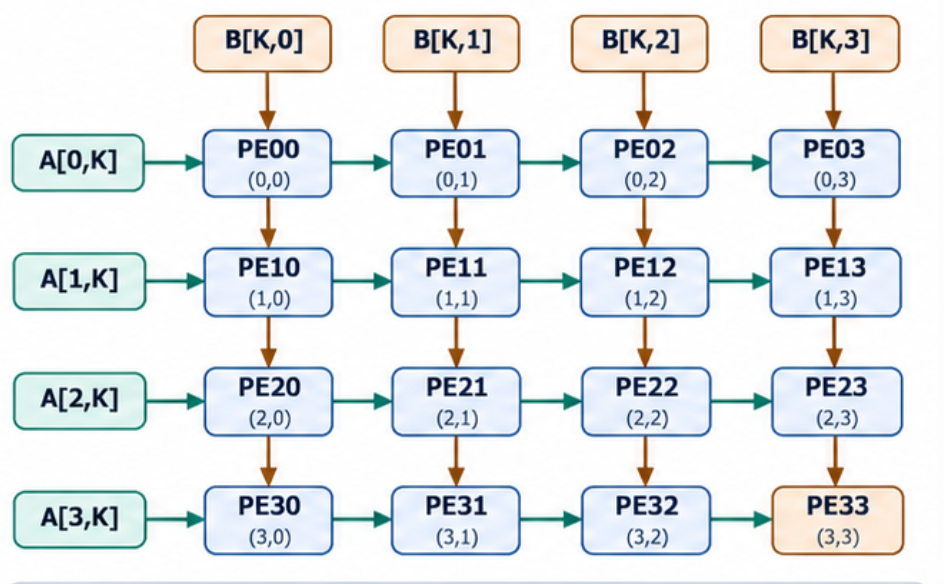
\includegraphics[width=0.8\linewidth]{figures/Systolic_flow.png}
    \caption{Luồn nhận tile của PE của Systolic array}
    \label{fig:placeholder}
\end{figure}

    Mỗi tile đã đọc từ BRAM được sử dụng tại bốn PE. Sau bốn lượt \textit{K}, hệ thống đã đọc 16 tile \textit{A} và 16 tile \textit{B}, tương ứng 128 phần tử đầu vào. Đây là lượng dữ liệu đọc từ hai BRAM đầu vào. Việc chuyển tiếp giữa các PE và truy cập RAM tổng riêng \textit{C} diễn ra bên trong mảng.

    \item \textbf{Lưu đồ thuật toán và FSM}

    Thuật toán bắt đầu tại ($K=0$). Trong mỗi lượt, hệ thống chuẩn bị bốn cặp tile, phát dữ liệu theo lịch và cập nhật tổng riêng tại từng PE. Ở lượt đầu, mỗi PE dùng tích đầu tiên của từng vị trí để khởi tạo tổng. Ở các lượt sau, PE tiếp tục cộng vào giá trị đã lưu. Bộ điều khiển chỉ tăng \textit{K} sau khi nhận đủ tín hiệu hoàn thành từ 16 PE. Sau lượt ($K=3$), hệ thống lần lượt xuất 64 phần tử kết quả theo thứ tự hàng.
    
\begin{figure}[H]
        \centering
        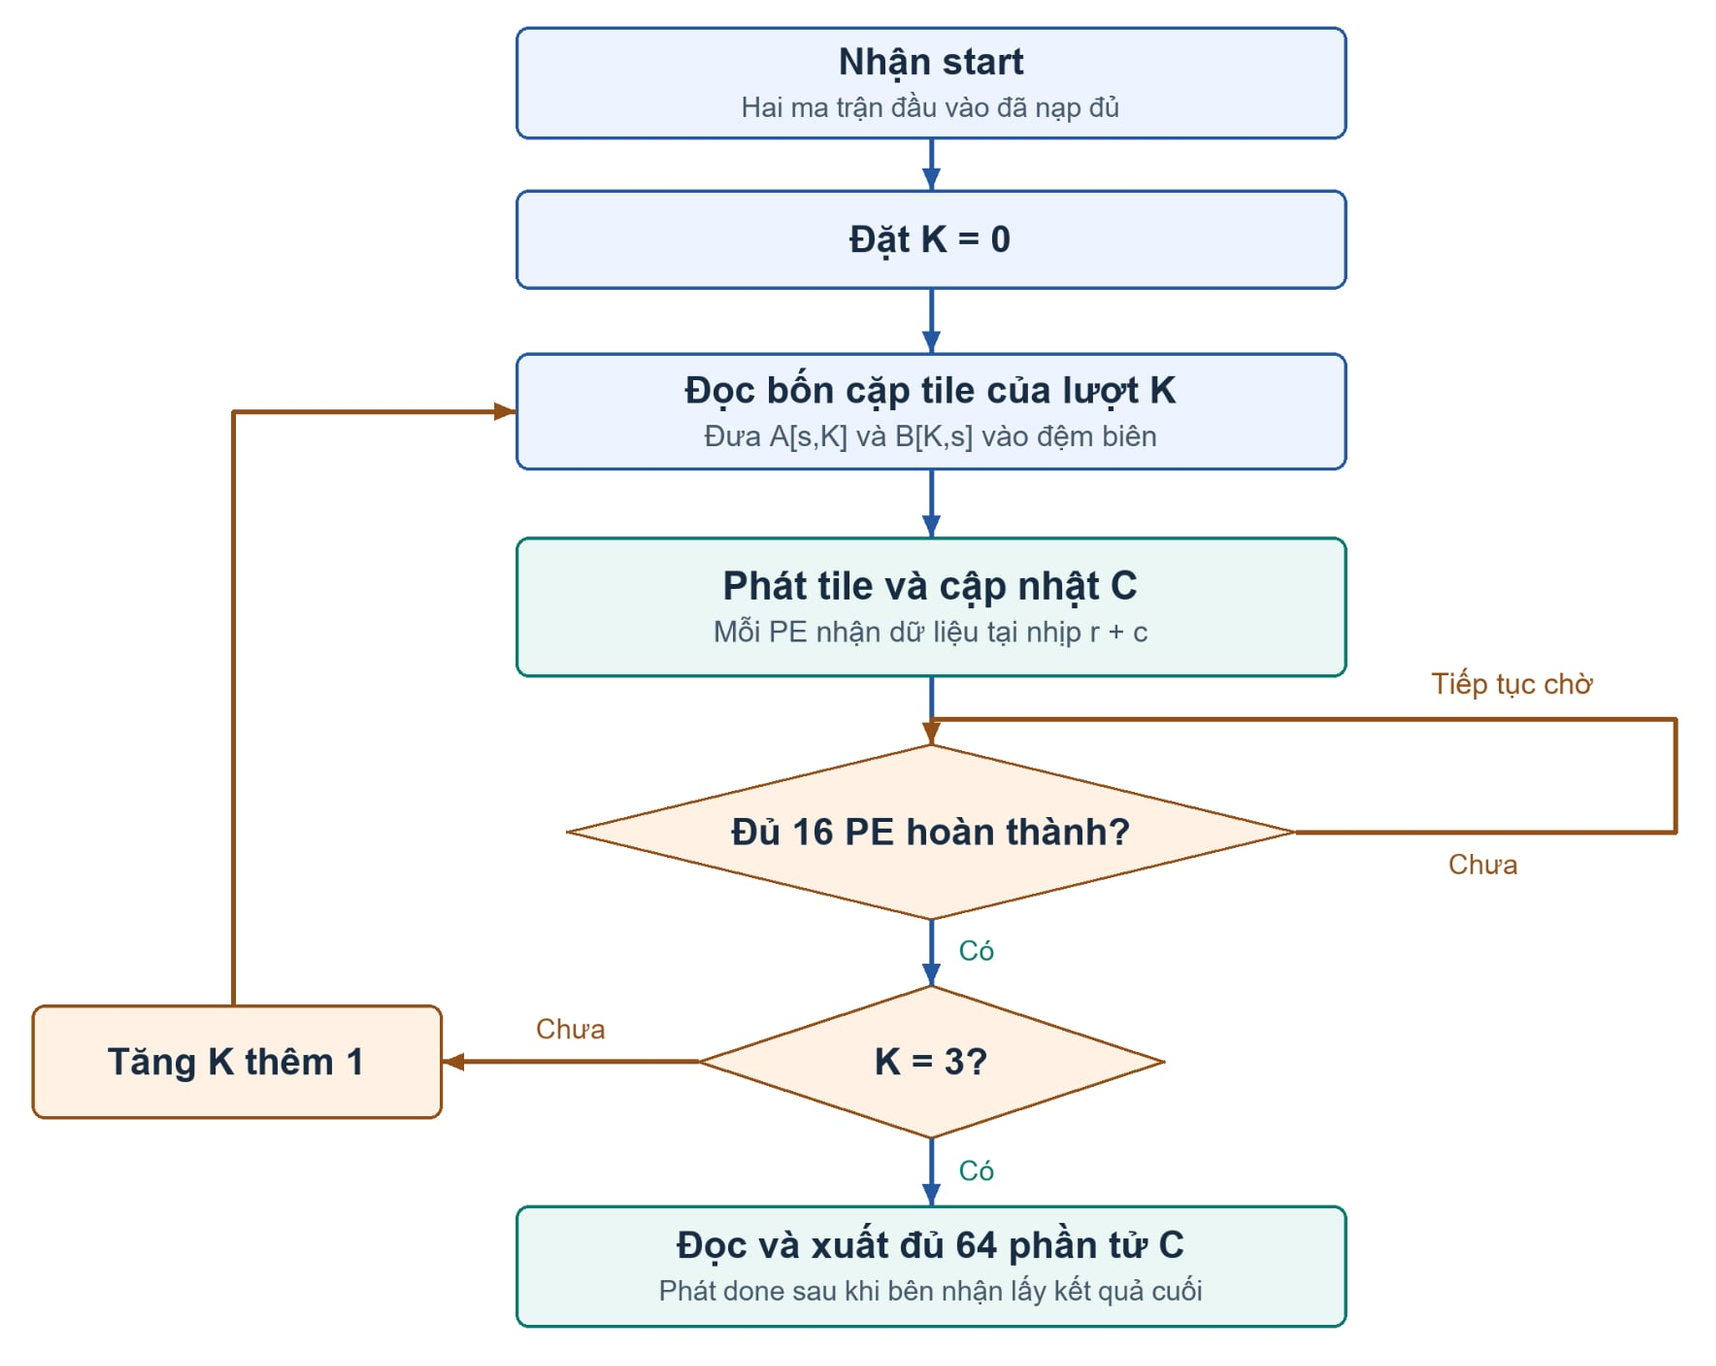
\includegraphics[width=0.8\linewidth]{figures/Systolic_flowchart.png}
        \caption{Lưu đồ thuật toán nhận ma trận theo luồng Systolic}
        \label{fig:placeholder}
\end{figure}

\begin{figure}[H]
    \centering
    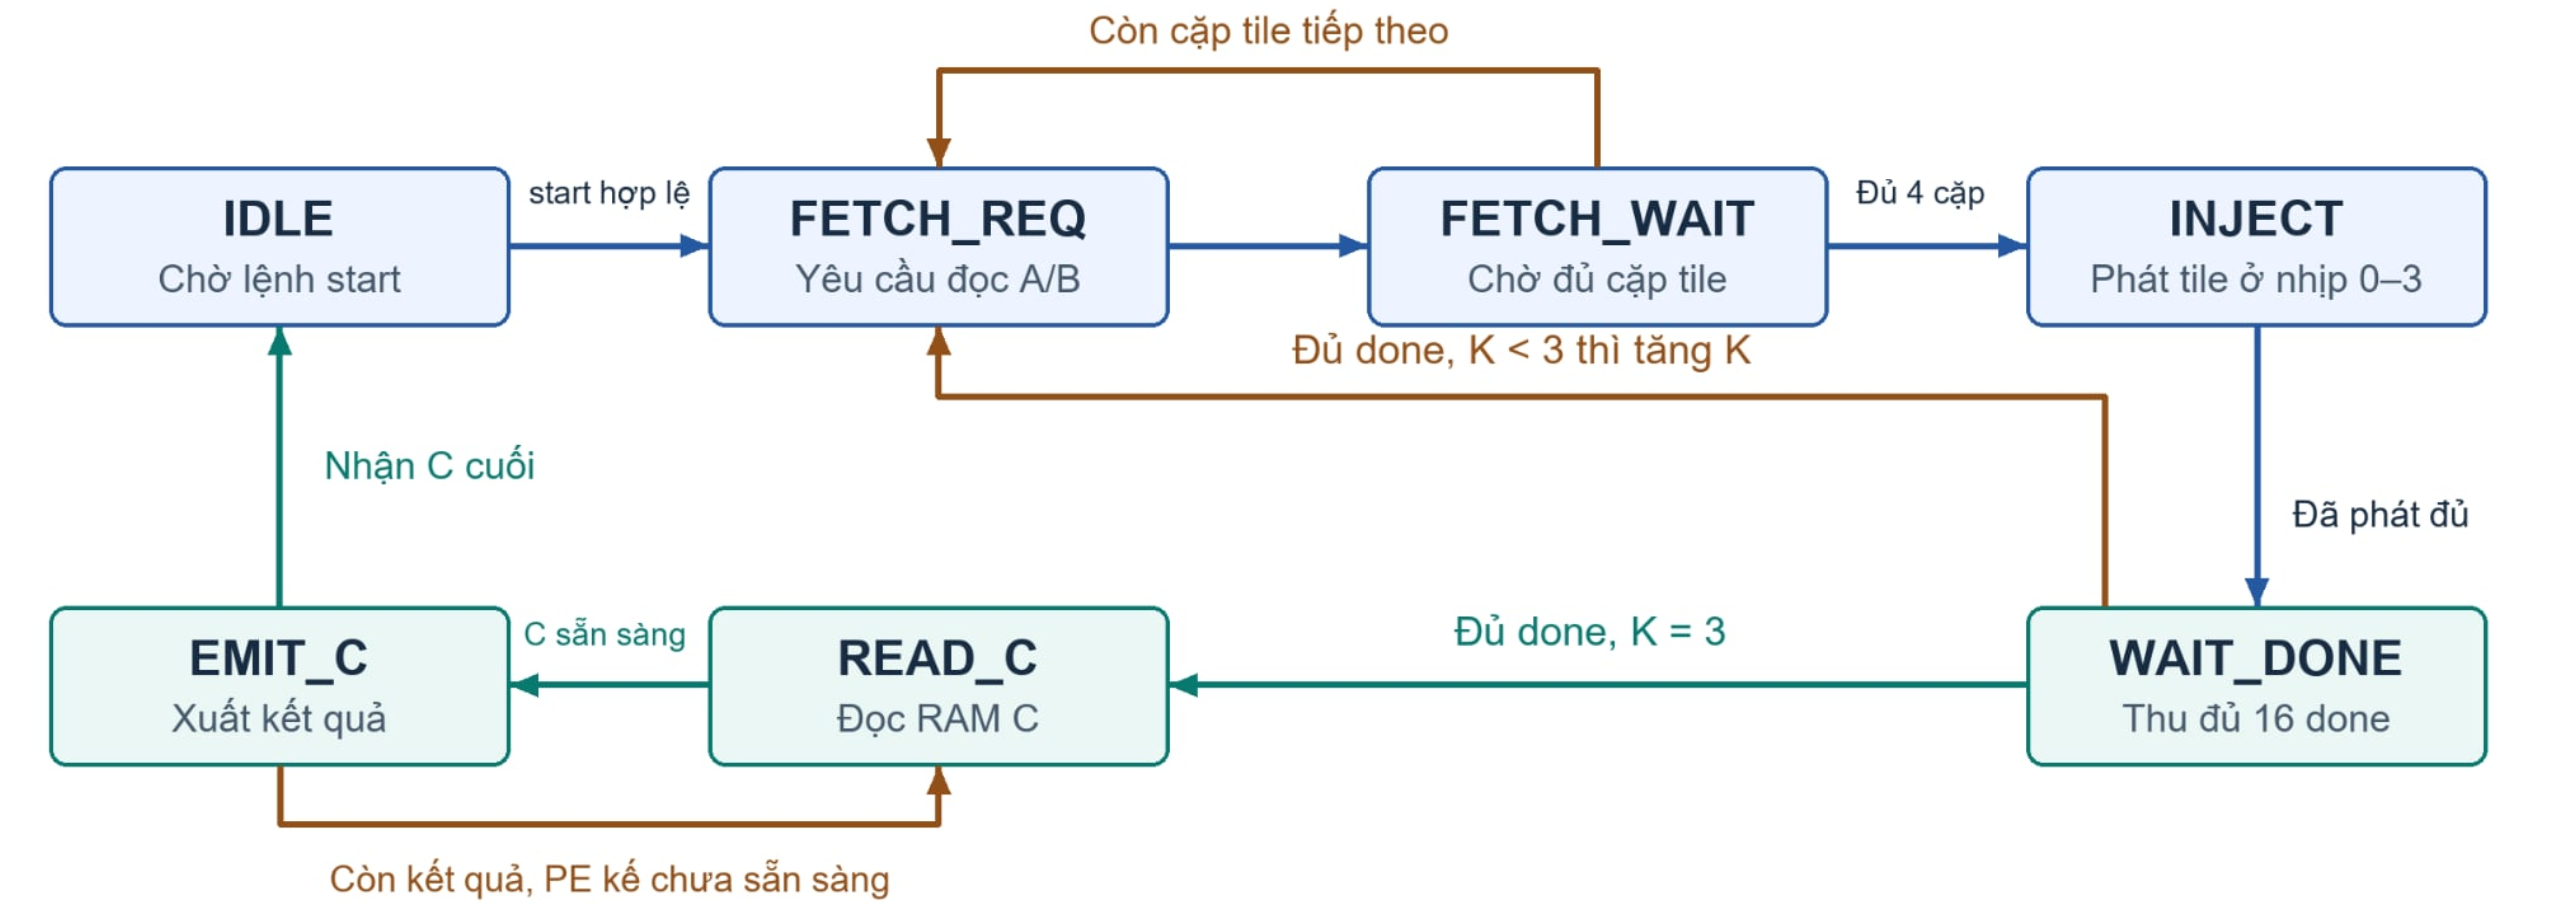
\includegraphics[width=1.0\linewidth]{figures/Systolic_FSM.png}
    \caption{FSM bộ nhân ma trận Systolic}
    \label{fig:placeholder}
\end{figure}
        
\end{enumerate}

\subsubsection{Phiên bản 2 - Multicast}
